%\documentclass[10pt]{article}
%\usepackage[utf8]{inputenc}
%\usepackage[english]{}

%\usepackage{color} %For interrogation about report or code
%\usepackage{hyperref} %Liens hypertexte du sommaire
%\usepackage{listings}
%\usepackage{moreverb}
%\usepackage{verbatim}
%\usepackage{graphicx} %To include image

%\title{Trampoline on LEGO MINDSTORMS NXT2 (from zero)}
%\author{Florent PAVIN}

%
%\begin{document}

%\maketitle
%\tableofcontents

%\newpage

\chapter{Trampoline on NXT}

%%%%%%%%%%%%%%%%%
%\section{Introduction}
This document describes how to get started a Trampoline \footnote{Trampoline is an open source RTOS which, once certified, could be compliant with the OSEK/VDX specification. Currently it is not the case, so while Trampoline has the same API as OSEK/VDX, it is not officially compliant. Trampoline is available under the GNU Lesser General Public License V2 and \textbf{is maintained by gcc-4.0.1}. Trampoline runs on several platforms like POSIX, C166 with Keil compiler, Star12X (courtesy of Geensys), PowerPC, ARM (NXT2 for example)} application on Lego Mindstorms NXT2.\\
The following steps will be overviewed :
\begin{itemize}
\item Trampoline installation
\item GCC compilation for ARM platform
\item Installation of drivers and softwares to be able to upload programs on the NXT.
\end{itemize}
This document is explained from a UNIX side. If you are on a Windows system, download and install Cygwin as it is explained on NXTOSEK website (\href{http://lejos-osek.sourceforge.net/installation_windows.htm}{http://lejos-osek.sourceforge.net/installation\_windows.htm}) first.

%%%%%%%%%%%%%%%
\section{Trampoline}
To download Trampoline, type in a terminal :
	\begin{verbatim}
	$svn checkout https://trampoline.rts-software.org/svn/trunk
	\end{verbatim}
Download the libpm (\href{http://galgas.rts-software.org/download/}{http://galgas.rts-software.org/download/}) for your achitecture and copy it in trunk/.\\
To compile GOIL, go in goil/makefile\_[ARCH] depending on your architecture and type in a terminal (you can add -j2 if you have 2 processors) :
	\begin{verbatim}
	$make goil
	\end{verbatim}
This will generate the GOIL executable you'll need. You can add the path to your GOIL (in $\sim$/.profile), adding :
	\begin{verbatim}
	export PATH=[TRAMPOLINE_REPOSITORY]/goil/makefile_[ARCH]/:$PATH
	\end{verbatim}

You can now use Trampoline on Unix system by executing the tests as described in Annex \ref{tests}.

%%%%%%%%%%%%%%%%
\section{GNUARM}
Download and unpack the necessary packages: binutils, gcc, newlib and gdb.
\begin{verbatim}
$ mkdir ~/crossgcc && cd ~/crossgcc
$ wget ftp://sourceware.org/pub/binutils/snapshots/binutils-2.18.50.tar.bz2
$ tar jxf binutils-2.18.50.tar.bz2
$ wget http://ftp.gnu.org/pub/gnu/gcc/gcc-4.2.3/gcc-4.2.3.tar.bz2
$ tar jxf gcc-4.2.3.tar.bz2
$ wget ftp://sources.redhat.com/pub/newlib/newlib-1.16.0.tar.gz
$ tar zxf newlib-1.16.0.tar.gz
$ wget http://ftp.gnu.org/pub/gnu/gdb/gdb-6.6.tar.gz
$ tar zxf gdb-6.6.tar.gz
\end{verbatim}

The installation directory should be /usr/local/crossgcc.

\begin{verbatim}
$ sudo mkdir /usr/local/crossgcc
$ sudo chmod 777 /usr/local/crossgcc
\end{verbatim}

First we build the binutils:

\begin{verbatim}
$ mkdir build-binutils && cd build-binutils
$ ../binutils-2.18.50/configure --target=arm-elf \
--prefix=/usr/local/crossgcc/ 2>&1 | tee configure.log
$ make all install 2>&1 | tee make.log
$ export PATH=$PATH:/usr/local/crossgcc/bin
\end{verbatim}

Build the gcc compiler with C/C++ support:

\begin{verbatim}
$ cd ../gcc-4.2.3
$ ln -s ../newlib-1.16.0/newlib .
$ ln -s ../newlib-1.16.0/libgloss .
$ cd ..
$ mkdir build-gcc && cd build-gcc
$ ../gcc-4.2.3/configure --target=arm-elf \
--prefix=/usr/local/crossgcc/ --with-newlib \
--with-gnu-as --with-gnu-ld --enable-languages=c,c++ 2>&1 | tee configure.log
$ make all install 2>&1 | tee make.log
\end{verbatim}

Build the gdb debugger:

\begin{verbatim}
$ cd ..
$ mkdir build-gdb && cd build-gdb
$ ../gdb-6.6/configure --target=arm-elf --prefix=/usr/local/crossgcc/
$ make all install 2>&1 | tee make.log
\end{verbatim}

You can now compile an application for ARM as described in Annex \ref{compileanapplication}.

%%%%%%%%%%%%%%%%%%%%%%%%%
\section{Nexttool + Lego Drivers} \label{drivers}
%%%%%%
\subsection{MAC OS}
Download and install the Lego Drivers (\href{http://mindstorms.lego.com/en-us/support/files/default.aspx#Driver}{http://mindstorms.lego.com/en-us/support/files/default.aspx
\#Driver}) and the firmware update (\href{http://mindstorms.lego.com/en-us/support/files/default.aspx#Firmware}{http://mindstorms.lego.com/en-us/support/files/default.aspx\#Firmware}) for MAC OS. \\
Download Nexttool (\href{http://bricxcc.sourceforge.net/utilities.html}{http://bricxcc.sourceforge.net/utilities.html}) and a new firmware (\href{http://bricxcc.sourceforge.net/lms_arm_jch.zip}{http://bricxcc.sourceforge.net/lms\_arm\_jch.zip}) and update the firm-ware as explained below :
\begin{itemize}
\item Reset the NXT : To go into firmware update mode, press the reset button (at the back of the NXT, upper left corner beneath the USB connector) for more than 5 seconds while the NXT is turned on. The NXT will audibly tick when it is in firmware update mode.
\item Copy an Enhanced NXT firmware (i.e. lms\_arm\_nbcnxc\_107.rfw) to NeXTTool extracted directory.
\item Launch Nexttool, and updload the Enhanced NXT firmware to the NXT (clicking on "Download firmware"), selecting it.
	\begin{figure}[h] %  figure placement: here, top, bottom, or page
   		\centering
		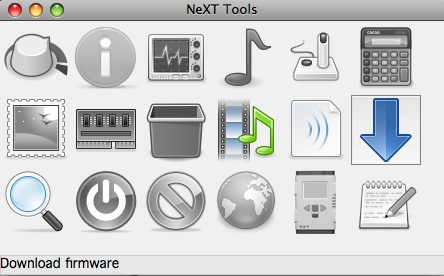
\includegraphics[width=0.7\textwidth]{pictures/firmware.jpg}
	\end{figure}
\item Remove the battery from the NXT and insert it again, and then press orange rectangle button on the NXT to turn on the Enhanced NXT firmware. The Enhanced NXT firmware has same GUI as the LEGO standard firmware.
\end{itemize}
To upload a program into the NXT, go to the Annex \ref{uploadprogram}.

%%%%
\subsection{Linux}
Follow the instructions in the NXTOSEK website \href{http://lejos-osek.sourceforge.net/installation_linux.htm}{http://lejos-osek.sourceforge.n et/installation\_linux.htm}.

%%%%
\subsection{Windows}
Download and install the Lego Drivers (\href{http://mindstorms.lego.com/en-us/support/files/default.aspx#Driver}{http://mindstorms.lego.com/en-us/support/files/default.aspx
\#Driver}) for PC. \\
Download Nexttool (\href{http://bricxcc.sourceforge.net/nexttool.zip}{http://bricxcc.sourceforge.net/nexttool.zip}) and a new firmware (\href{http://bricxcc.sourceforge.net/lms_arm_jch.zip}{http://bricxcc.sourceforge.net/lms\_arm\_jch.zip}) and update the firm-ware as explained below :
\begin{itemize}
\item Reset the NXT : To go into firmware update mode, press the reset button (at the back of the NXT, upper left corner beneath the USB connector) for more than 5 seconds while the NXT is turned on. The NXT will audibly tick when it is in firmware update mode.
\item Copy an Enhanced NXT firmware (i.e. lms\_arm\_nbcnxc\_107.rfw) to NeXTTool extracted directory.
\item Execute Cygwin and type the following command to change the current directory to the NexTTool extracted directory. (NeXTTool is assumed to be extracted under C:$\backslash$cygwin$\backslash$nexttool directory)
	\begin{verbatim}
	$cd C:\cygwin\nexttool
	\end{verbatim}
\item Connect PC and the NXT by USB cable.
\item Type the following command in Cygwin to upload the Enhanced NXT firmware to the NXT (Program upload may take around half minutes and then, NXT LCD is turned to display some chunk from blank).
	\begin{verbatim}
	$./NeXTTool.exe /COM=usb -firmware=lms\_arm\_nbcnxc\_107.rfw
	\end{verbatim}
\item Remove the battery from the NXT and insert it again, and then press orange rectangle button on the NXT to turn on the Enhanced NXT firmware. The Enhanced NXT firmware has same GUI as the LEGO standard firmware.
\end{itemize}
You can now upload a program into the NXT as described in the Annex \ref{uploadprogram}.

\newpage
\chapter{Appendix}
%%%%%%%%%%%%%%%%%%%%%%%%%
\section{Launching Trampoline tests} \label{tests}
To launch the tests you have to compile ViPER \footnote{Virtual Processor Emulator, ViPER is used on Posix system to send interrupts to Trampoline to emulate the timers. It is launched by Trampoline.} first. Go in viper/ and type in a terminal :
	\begin{verbatim}
	$make
	\end{verbatim}
To launch the tests, go in check/ and type in a terminal :
	\begin{verbatim}
	$./tests.sh
	\end{verbatim}
At the end of the tests you should see :
	\begin{verbatim}
	...
	Compare results with the expected ones...
	Functional tests Succeed!!
	GOIL tests Succeed!!
	\end{verbatim}
If an error occurs, you can visit Trampoline's forum (\href{http://trampoline.rts-software.org/bb/}{http://trampoline.rts-software.org/bb/}).


%%%%%%%%%%%%%%%%%%%%%%%%%
\section{Cross-Compile an application} \label{compileanapplication}
To cross-compile a Trampoline application for ARM ports, you need to set  :
\begin{itemize}
\item COMPILER = "arm-elf-gcc";
\item ASSEMBLER = "arm-elf-as";
\item LINKER = "arm-elf-ld";
\end{itemize}
in your oil file as you can see in examples/arm/nxt/lonely.oil.\\
And then, compile your application typing in a terminal (from the example in examples/arm/nxt) :
	\begin{verbatim}
	$goil -t=arm/nxt --templates=../../../goil/templates -g -i lonely.oil
	$make
	\end{verbatim}
Then you need to upload the *.rxe file (see Annex \ref{uploadprogram}- after installing drivers and softwares on your platform (\ref{drivers})

%%%%%%%%%%%%%%%%%%%%%%%%%
\section{Upload a program} \label{uploadprogram}
\subsection{MAC OS}
To upload a program in the NXT (the nxt example examples/arm/nxt/lonely\_exe.rxe)
\begin{itemize}
\item Connect the PC and the NXT by USB cable.
\item Launch Nexttool, select "usb port".
	\begin{figure}[htbp] %  figure placement: here, top, bottom, or page
   		\centering
		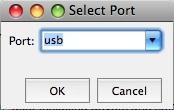
\includegraphics[width=0.25\textwidth]{pictures/usbport.jpg}
	\end{figure}
\item Go to "NXT Explorer"
	\begin{figure}[htbp] %  figure placement: here, top, bottom, or page
   		\centering
		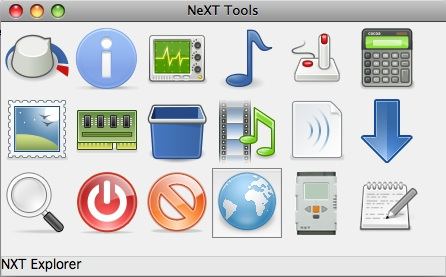
\includegraphics[width=.7\textwidth]{pictures/nxtexplorer.jpg}
	\end{figure}
\item Click on the "Download selected files to the NXT" and select the lonely\_exe.rxe file.
\item If program upload was succeeded, you can see the lonely\_exe.rxe file in the files list as below.
	\begin{center}[h] %  figure placement: here, top, bottom, or page
   		%\centering
		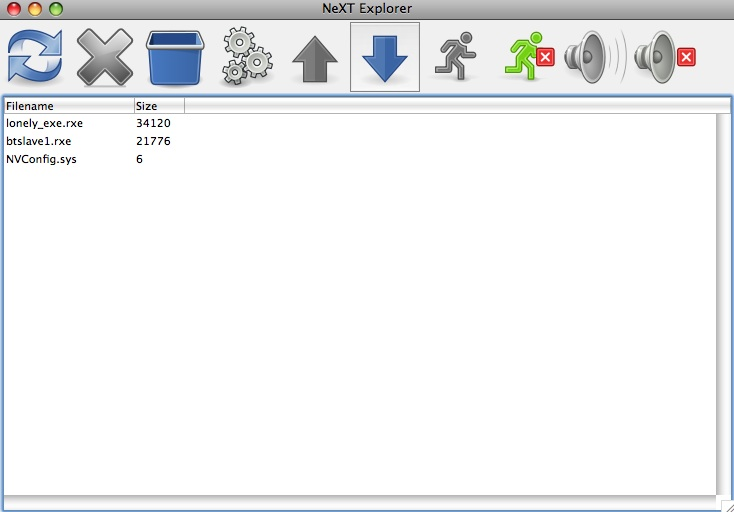
\includegraphics[width=1\textwidth]{pictures/downloadfile.jpg}
	\end{center}
\item To execute a program on the NXT, go in "My files"/"Software files".
\end{itemize}

%%%%
\subsection{Linux}
Follow the instructions in the NXTOSEK website \href{http://lejos-osek.sourceforge.net/installation_linux.htm}{http://lejos-osek.sourceforge.net/installation\_linux.htm}.

%%%%
\subsection{Windows}
To upload a program in the NXT (the nxt example examples/arm/nxt/lonely\_exe.rxe) follow the steps below :
\begin{itemize}
\item Connect the PC and the NXT by USB cable.
\item Type the following command in Cygwin (from examples/arm/nxt) :
	\begin{verbatim}
	$wine NeXTTool.exe /COM=usb -download=lonely_exe.rxe
	$wine NeXTTool.exe /COM=usb -listfiles=lonely_exe.rxe
	\end{verbatim}
\item If program upload was succeeded, program size could be displayed in Cygwin such as the second line in the below command outputs. 
	\begin{verbatim}
	Executing NeXTTool to upload helloworld.rxe...
	helloworld.rxe=15280
	NeXTTool is terminated.
	\end{verbatim}
\item To execute a program on the NXT, go in "My files"/"Software files".
\end{itemize}

%\end{document}

